% Author: Marco Miani
\documentclass[varwidth=true, border=2pt]{standalone}

\usepackage{pgfplots}
\pgfplotsset{compat=1.9}

\begin{document}
    \pgfplotsset{
        colormap={whitered}{
            color(0cm)=(white);
            color(1cm)=(orange!75!red)
        }
        %colormap={color}{color(0cm)=(white); color(1cm)=(blue)}
    }
    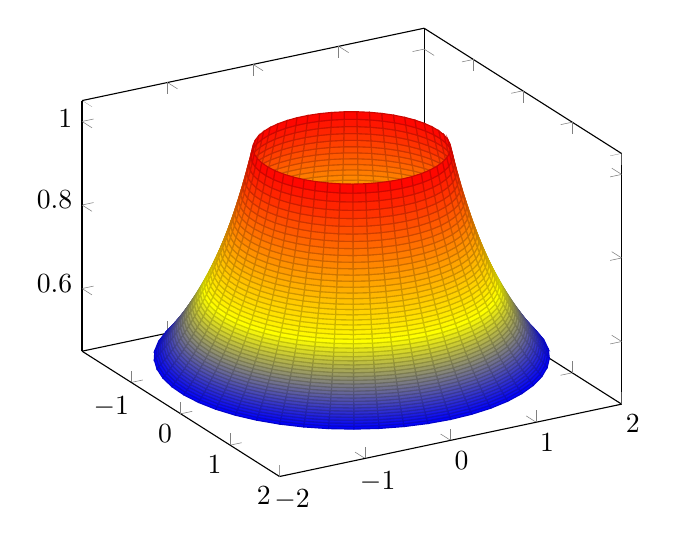
\begin{tikzpicture}
     \begin{axis}[view={60}{30}]
      \addplot3[surf,
      samples=50,
      domain=1:2,y domain=0:2*pi,
      z buffer=sort]
      %({(2 + tan(deg(y)))*cos((deg(x)))}, {(2 + cos(x)) * sin(x)}, {x});
      ({x * cos(deg(y))}, {x * sin(deg(y))}, {1/x});
     \end{axis}
    \end{tikzpicture}
\end{document}
